\section{Contextual Analyzer}
	This section will explain how type checking and scope checking is performed on the AST which was constructed from the parser.
	To do this a way of traversing the tree is needed, in which we chose the Visitor Pattern.
	
	\subsection{Visitor Pattern}
		\label{impl:visitorinterface}
		The Visitor Pattern is a design pattern used to traverse tree structures. 
		The design pattern is a smart way of separating traversal of the tree and the code that has to be executed at the tree nodes. \\
		This is done by making a {\it Visitor interface} that has a {\it Visit method} for each of the nodes that 
		can be visited (See figure \ref{impl:visitor}). Classes that wish to traverse the tree can then implement the interface and its methods.
		\begin{figure}[H]
		\center
			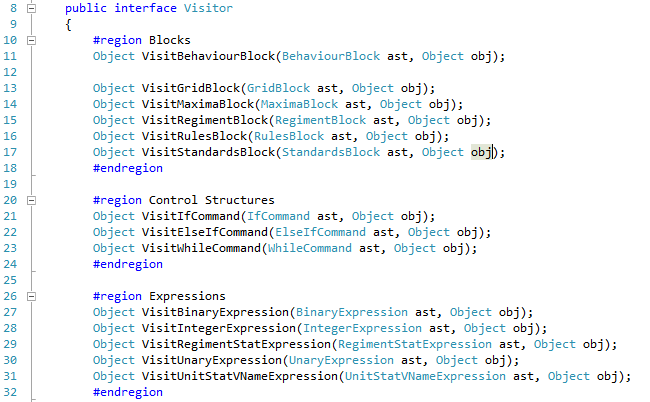
\includegraphics[scale=0.8]{rapport/6/figures/visitorinterface.png}
			\caption{Screenshot of some of the Visitor interface}
			\label{impl:visitor}
		\end{figure}
	
		The class nodes will all have a {\it Visit method}, 
		which is overridden from the AST class, that calls the method from the visitor class 
		that corresponds to the node (See figure \ref{impl:visitnode}). 
			\begin{lstlisting}[basicstyle=\small\sffamily,
					keywords={break,case,const,continue,default,else,enum,
					for,if,return,switch,while,do,long,void,int,float,double,
					char,struct,typedef,include,size\_t},
					keywordstyle={\color{blue}},
					comment={[l]{//}}, morecomment={[s]{/*}{*/}}, commentstyle=\itshape,
					columns={[l]flexible}, numbers=left, numberstyle=\tiny,
					frameround=fftt, frame=shadowbox, captionpos=b,
					caption={Example of a node class with a Visit method},
					label=impl:visitnode]
class TreeNode:AST
{
	public Node a,b;
	public TreeNode(Node a, Node b)
	{
		this.a = a;
		this.b = b;
	}
	public Visit(Visitor v, object arg)
	{
		//Calls the right visit method from the visitor class
		v.VisitTreeNode(this,arg);
	}
}
			 \end{lstlisting}
	
	\subsection{Checker class}
		The {\it Checker class} implements the Visitor interface seen in \ref{impl:visitor}. 
		In its visit methods it checks for type rules and scope rules. 
		To keep track of the current scope level and of declarations we use an {\it Identification table}.
		
		\subsubsection{Identification table}
			The identification table is a class named {\it IdentificationTable}(see \ref{impl:idtable}), which contains a list with entries 
			that holds the information declarations made and an integer {\it level} that represents the current scope level. 
			For adding and retrieving entries {\it EnterEntry} and {\it RetrieveEntry} are used.
			For opening and closing the current scope {\it Open} and {\it Close}. Open increases the {\it level} and Close removes 
			all the declarations made on the current level and {\it level} decreases it by one.
			\begin{lstlisting}[basicstyle=\small\sffamily,
					keywords={break,case,const,continue,default,else,enum,
					for,if,return,switch,while,do,long,void,int,float,double,
					char,struct,typedef,include,size\_t},
					keywordstyle={\color{blue}},
					comment={[l]{//}}, morecomment={[s]{/*}{*/}}, commentstyle=\itshape,
					columns={[l]flexible}, numbers=left, numberstyle=\tiny,
					frameround=fftt, frame=shadowbox, captionpos=b,
					caption={The IdentificationTable class},
					label=impl:idtable]
class IdentificationTable
{
	private int level=0;
	private List<IdEntry> entries = new List<IdEntry>();
	
	public void Open(){}
	public void Close(){}
	
	public bool EnterEntry(Declaration declaration,string id){}
	public Declaration RetrieveEntry(string id){}
}
			\end{lstlisting}	
		
		\subsubsection{Scope Rules checking}
			For opening and closing the current scope we use the {\it IdentificationTable class} just described.
			When we are entering a new scope the {\it Open method} is called and when we are leaving the scope the {\it Close method} is called.
			Here is the {\it VisitRegimentBlock method} which needs to open and close scopes: \\
			\begin{lstlisting}[basicstyle=\small\sffamily,
					keywords={break,case,const,continue,default,else,enum,
					for,if,return,switch,while,do,long,void,int,float,double,
					char,struct,typedef,include,size\_t},
					keywordstyle={\color{blue}},
					comment={[l]{//}}, morecomment={[s]{/*}{*/}}, commentstyle=\itshape,
					columns={[l]flexible}, numbers=left, numberstyle=\tiny,
					frameround=fftt, frame=shadowbox, captionpos=b,
					caption={The IdentificationTable class},
					label=impl:idtable]
public Object VisitRegimentBlock(RegimentBlock ast, Object obj)
{
	//Opening scope
	idTable.Open();
	
	//Visits children
    ast.bn.Visit(this, null);
    ast.usds.ForEach(x => x.Visit(this, null));
    ast.bb.Visit(this, null);
    
    //Closing scope
    idTable.Close();
    
	return null;
}
			 \end{lstlisting}
		
		\subsubsection{Type checking}			
			When the checker visits a node where type checking is needed (e.g. RegimentStat), the checker visits the nodes 
			in need of identification. Here the datatype of the node is retrieved from the identification table, if the datatype matches the 
			expected datatype, it simply proceeds, else it reports an error and then proceeds. \\
\begin{lstlisting}[basicstyle=\small\sffamily,
					keywords={break,case,const,continue,default,else,enum,
					for,if,return,switch,while,do,long,void,int,float,double,
					char,struct,typedef,include,size\_t},
					keywordstyle={\color{blue}},
					comment={[l]{//}}, morecomment={[s]{/*}{*/}}, commentstyle=\itshape,
					columns={[l]flexible}, numbers=left, numberstyle=\tiny,
					frameround=fftt, frame=shadowbox, captionpos=b,
					caption={Type checking of RegimentStat},
					label=impl:typecheck]	
public Object VisitRegimentStat(RegimentStat ast, Object obj)
{
	ast.i.Visit(this, null);
	Declaration declaration = idTable.RetrieveEntry(ast.i.spelling);
	if (declaration == null)
	{
	reporter.ReportCheckerError("Regiment % wasn't declared", 
			ast.i.spelling, ast.i.position);
	}
	else if (ast.i.type != DataType.Regiment)
	{
	reporter.ReportCheckerError("% was not of type Regiment", 
			ast.i.spelling, ast.i.position);
	}
		ast.ust.Visit(this, null);
		return null;
    }
}
\end{lstlisting}
			This code snippets shows type checking for {\it RegimentStat}. 
			The production rule of RegimentStat is:
			\begin{equation}
				RegimentStat ::= Identifier.UnitStatType
			\end{equation} 
			This means that we have to check if the identifier has been declared and we have to check if the identifier is of type Regiment.
			These two checks can be seen above in the {\it if statement} and the {\it if else statement}. \\
			
			The type checking also serves another purpose called decoration. When a variable/constant is declared the data type 
			and the value of the variable/constant is saved. Each time the checker visits a node which references a declared 
			variable/constant it decorates it with its data type and value.
			When the type rules checking has finished the AST that is traversed is fully decorated.
			
			
		